\chapter{Justificativa da Abordagem}
\label{justify}

\section{Principais abordagens utilizadas no mercado}

Em desenvolvimento de \textit{software}, há as abordagens dos modelos preditivos e adaptativos. Cada modelo tem suas vantagens e desvantagens, se encaixando melhor em contextos determinados. Para a construção desse projeto, foram analisados os processos \textit{Rational Unified Process} (RUP) e \textit{Scaled Agile Framework} (SAFe) para verificação e otimização do mais adaptado ao contexto encontrado.

\section{Sobre o RUP - \textit{Rational Unified Process}}

O \textit{Rational Unified Process} é um processo de engenharia de \textit{software} que provê disciplinas e atribui tarefas e responsabilidades para uma organização desenvolvedora que procura um modelo visando qualidade e desenvolvimento iterativo.~\cite{kruchten}

\subsection{Estrutura do RUP}

A estrutura desse processo pode ser observada pela figura \ref{rup-phases}, onde:

\begin{itemize}
\item O eixo horizontal representa tempo e aspectos do ciclo de vida do projeto de \textit{software}
\item O eixo vertical representa as disciplinas implementadas no processo de \textit{software} e sua magnitude em cada etapa do ciclo de vida.
\end{itemize}

\begin{figure}[h]
\centering
  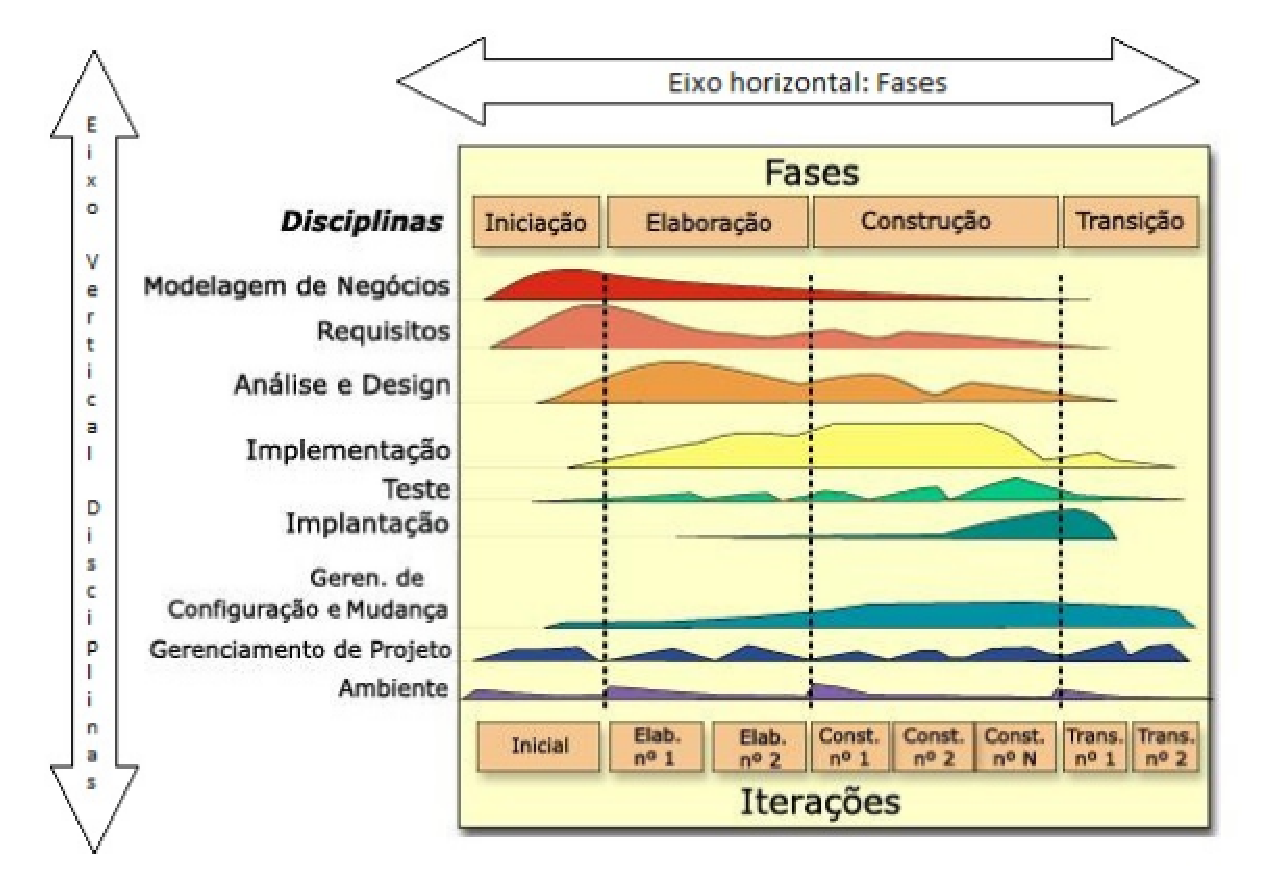
\includegraphics[keepaspectratio=true,scale=0.5]
  {figuras/fases_rup.eps}
  \caption{Gráfico das fases e iterações por disciplinas}
  \label{rup-phases}
\end{figure}

O processo unificado se divide nas seguintes fases:

\begin{itemize}
\item Iniciação: “Envolve tanto a atividade de comunicação com o clienta quanto a de planejamento. Colaborando com os interessados, identifica-se de negócio para o software; propõe uma arquitetura rudimentar e se desenvolve um planejamento para a natureza iterativa e incremental do projeto decorrente...”~\cite{pressman}
\item Elaboração: “Envolve atividades de comunicação e realização do modelo de processo genérico. A elaboração refina e expande os casos práticos preliminares desenvolvidos como parte da fase de iniciação, e amplia a representação da arquitetura...”~\cite{pressman}
\item Construção: “Tendo como entrada o modelo de arquitetura, a fase de construção desenvolve ou adquire componentes de software; esses componentes farão com que cada caso de uso se torne operacional para o usuário final. Então implementa-se, no código-fonte, todos os recursos e funções necessárias para o incremento do \textit{software}. À medida que os componentes estão sendo implementados, são desenvolvidos e executados testes unitários para cada um. Além disso, realizam-se atividades de integração…”~\cite{pressman}
\item Transição: “Abarca os últimos estágios da atividade de construção genérica e a primeira parte da atividade de emprego genérico: entrega e \textit{feedback}. O \textit{software} é entregado aos usuários finais para testes \textit{beta} são coletados seus \textit{feedbacks} para respectivas mudanças e erros encontrados. Além disso, a equipe de \textit{software} elabora material de apoio (manuais e guias, por exemplo) que são necessários para o lançamento da versão. Na conclusão da fase de transição, o incremento torna-se uma versão de \textit{software} utilizável.”~\cite{pressman}
\end{itemize}

\section{Sobre o SAFe - \textit{Scaled Agile Framework}}

A metodologia ágil existe desde a década de 80, porém foi pouco utilizada, dando espaço às metodologias tradicionais. Foi confundido seu foco nas pessoas com ausência de documentação. Por essa razão, muitos desenvolvedores achavam que a metodologia era descuidada, sem padrão ou documentos. Essa informação não é verídica e há exemplos de metodologia ágil bem sucedida na indústria, como por exemplo na Toyota, que adota uma linha de produção nesse modelo.~\cite{dev2}

O SAFe se baseia em princípios Lean e Ágeis para sintetizar o conhecimento obtido por gerações de \textit{deployments} de \textit{softwares} em um único \textit{framework}, fornecendo um conjunto integrado de atividades que têm demonstrado melhorar aspectos no desenvolvimento de \textit{software}, como por exemplo produtividade do time e qualidade da solução.~\cite{safe}

\begin{figure}[h]
\centering
  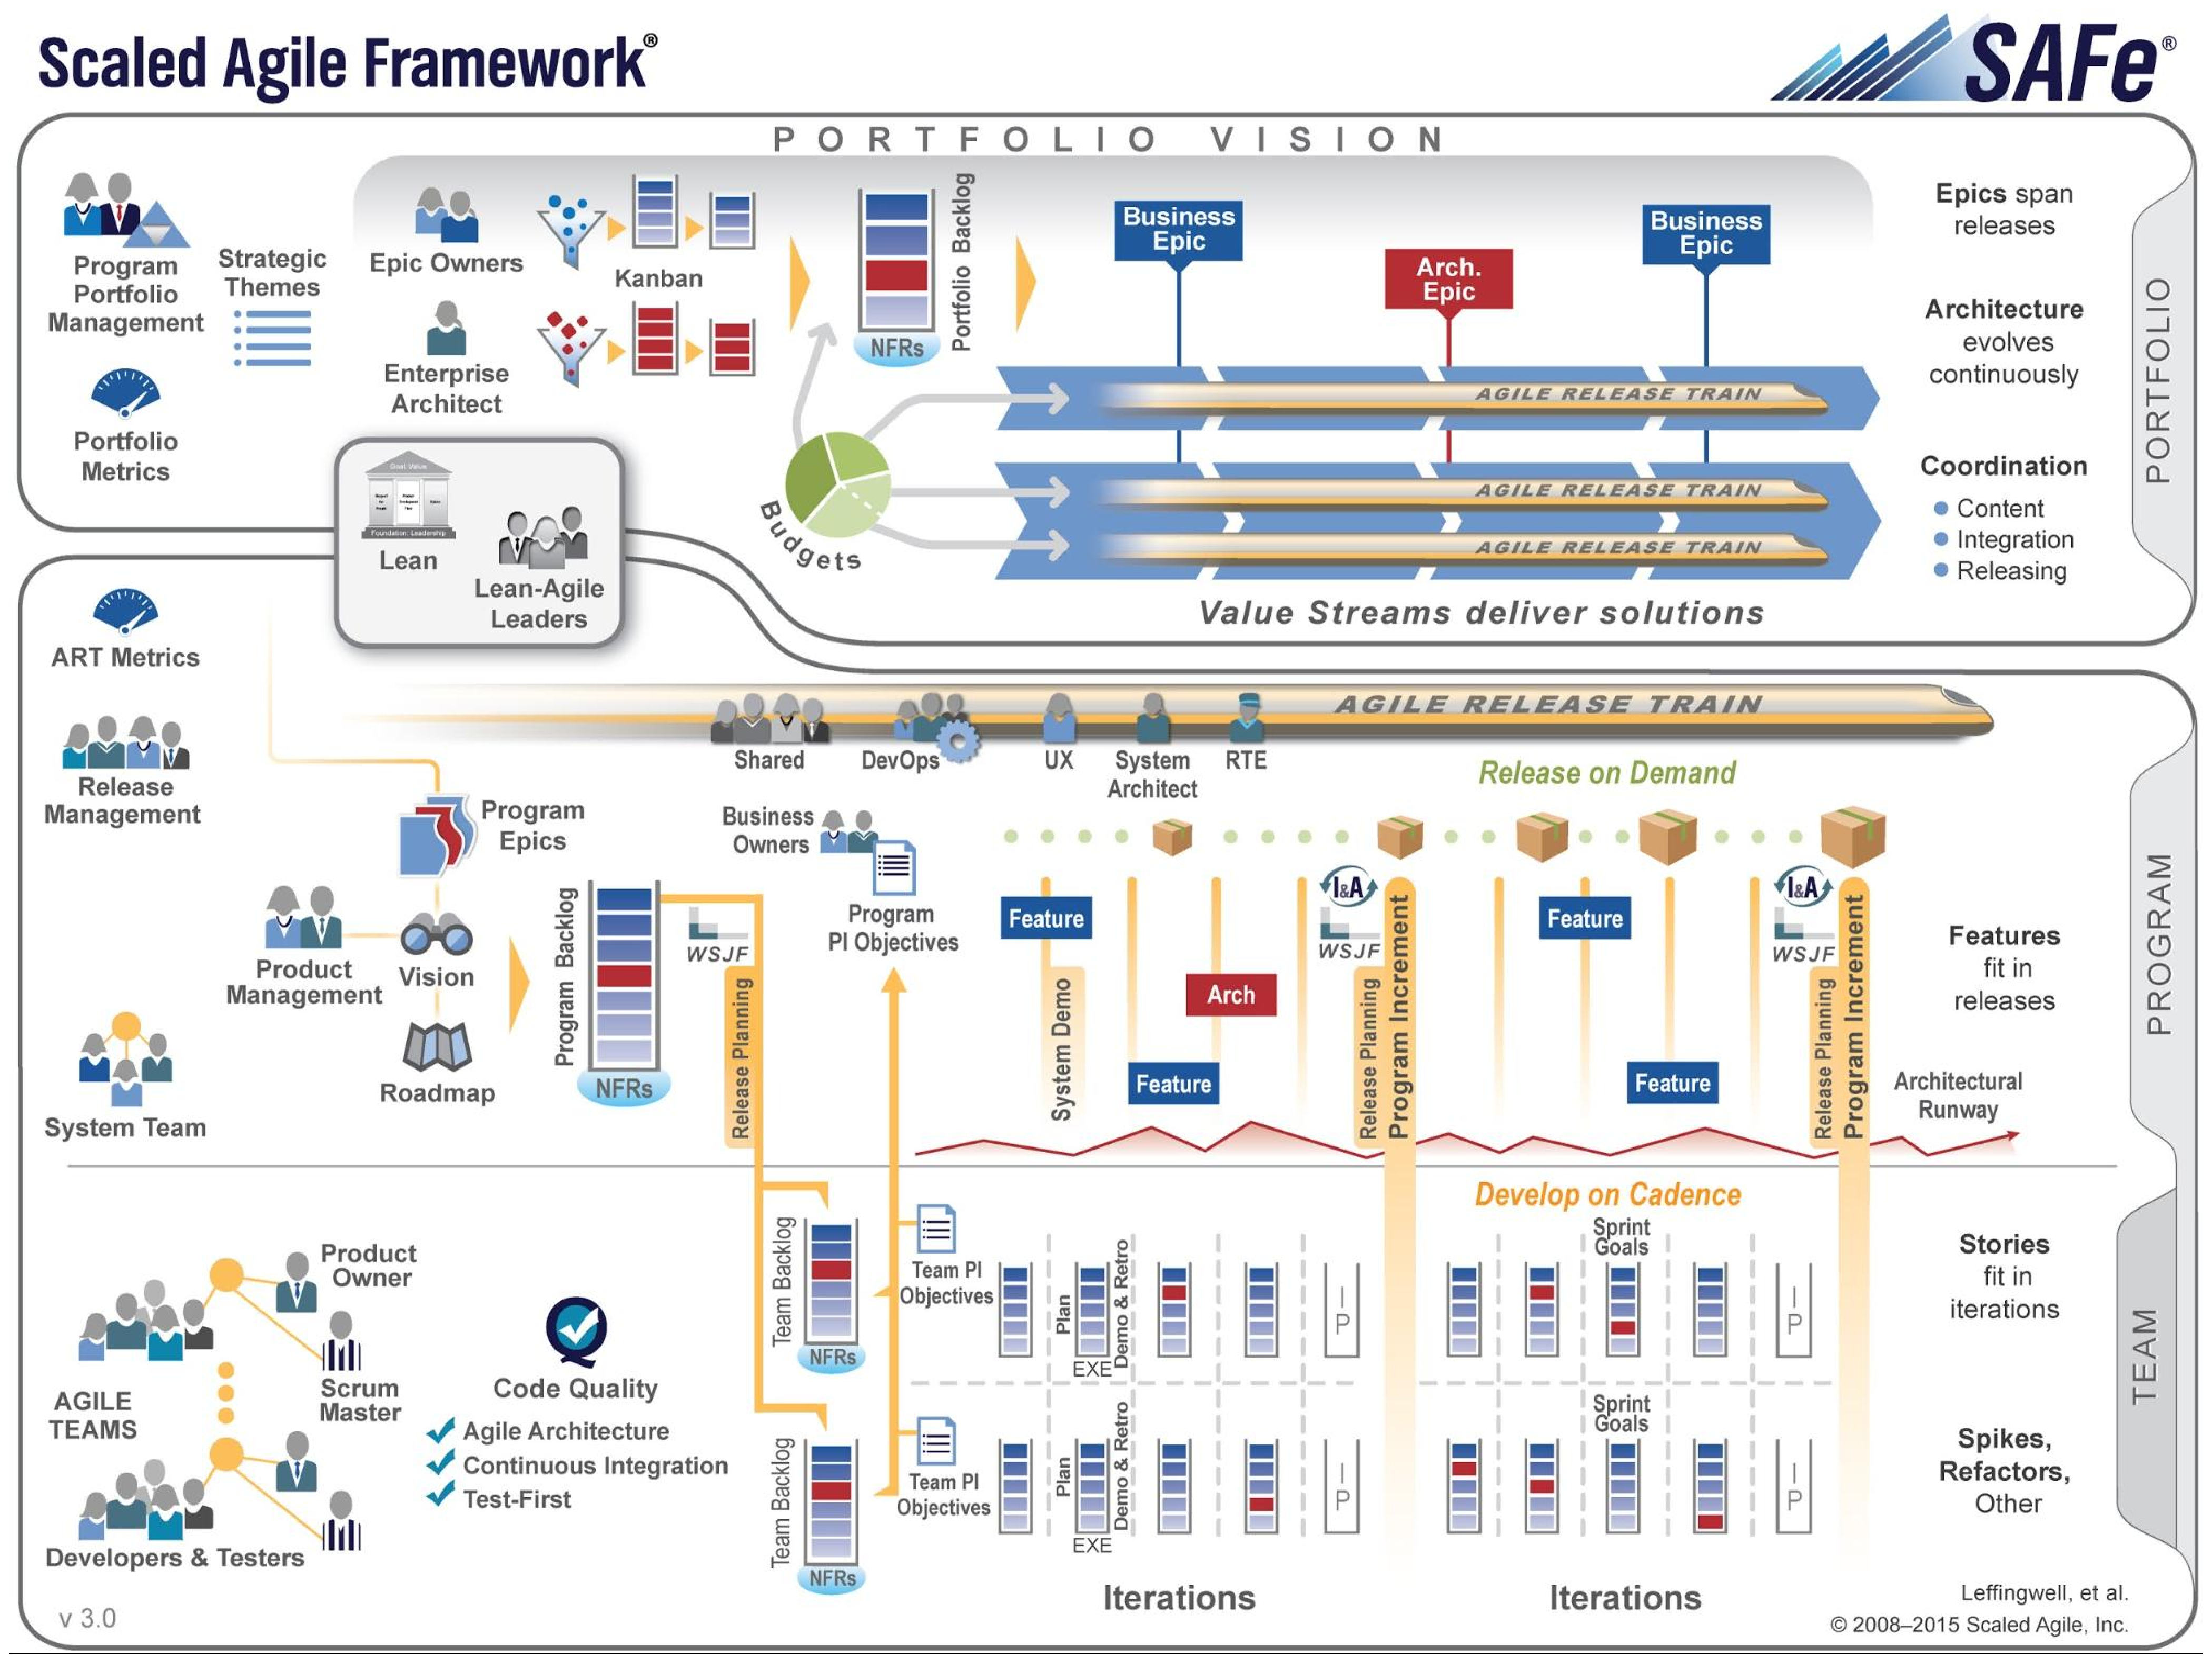
\includegraphics[keepaspectratio=true,scale=0.2]
  {figuras/safe.eps}
  \caption{\textit{Scaled Agile Framework}}
  \label{safe}
\end{figure}

Tendo como base a figura \ref{safe}, é possível perceber que as atividades associadas à requisitos no SAFe estão divididas em três visões:
\begin{description}
\item [Portfólio] É o nível mais alto do SAFe, onde estão alinhadas as estratégias de negócios e intenções de investimento da empresa. Nesse nível estão alguns pontos chaves, como: épicos, \textit{portfolio backlog} e métricas.~\cite{portfolio}
\item [Programa] Nível responsável por entregar frequentemente incrementos no programa, tipicamente entre 8-12 semanas em múltiplas iterações. Está associado, portanto, ao \textit{Agile Release Train}, que pode ser visto na figura \ref{safe}.~\cite{program}
\item [Time] Na visão de time, são fornecidas abstrações organizacionais para fornecer papéis e atividades que nortearão o desenvolvimento de \textit{software} em grandes empresas.~\cite{team}
\end{description}

\section{Abordagem escolhida}

Várias razões motivaram a optar pela a abordagem iterativa incremental baseada no \textit{Rational Unified Process}, descartando abordagens ágeis ou híbridas, sendo as mesmas:
\begin{itemize}
\item Em relação a abordagem ágil, a equipe possui pouca disponibilidade de tempo para realizar \textit{stand-ups} diários, retrospectiva, escrever histórias de usuários junto ao cliente, revisão com os \textit{stakeholders} e pareamento, principais práticas ágeis. Dessa forma, evita-se a utilização da metodologia ágil ou híbrida, pois haveria o prejuízo na adoção das mesmas.
\item Os integrantes da equipe se sentem mais confiantes quando estão sob uma metodologia de desenvolvimento com uma ampla utilização no mercado e documentação sobre suas práticas.
\item Como o \textit{Rational Unified Process} consiste em um modelo bem detalhado, facilitará um processo mais sutil da gerência de requisitos, pois nesse modelo a presença de documentos é incentivada.
\item A aborgadem híbrida foi evitada por ser concordado entre a equipe que é necessária experiência razoável para implantar os mecanismos das duas abordagens em um único processo de forma a conversarem harmonicamente. Mudanças simples como trocar histórias por casos de uso ou alguma outra troca de atividade não resultaria na integração e experiência desejadas para o desenvolvimento.
\item É predominante a abordagem iterativa incremental no mercado de trabalho de Brasília. Desse ponto de vista, é interessante utilizar a mesma para adquirir experiência.
\item Foi decidido a entrega de valor ao cliente através de documentos nas saídas das atividades com o propósito de: indicar que a atividade foi feita e para o cliente ter noção do andamento do projeto
\end{itemize}








